
\chapter{预备知识}

\begin{kaishu}

本章将要介绍的预备知识包括软件可信的相关理论,涵盖软件可信性的定义,软件属性、子属性和度量元,软件可信度量模型与分级方法。接着介绍结构方程模型的原理,以及系统开发所用到的框架与技术。
% 本章主要介绍的预备知识包括软件可信的相关理论,涵盖软件可信性的定义,软件属性、子属性和度量元,软件可信度量模型与分级方法。接着介绍结构方程模型的原理,以及系统开发所用到的框架与技术。

\end{kaishu}

\section{软件可信相关概念}
\subsection{软件可信性定义}
国内外学者和科研机构从不同的方面来定义软件可信性,目前学术界对软件可信性没有统一意见。

% 文献\cite{Schneider1999Trust}给出如果一个系统是可信的,即使在运行环境发生崩溃,操作人员出现操作错误、系统遭到恶意攻击、系统存在设计和实现错误的情况下,其也能够按照预期的方式运行。
文献\cite{陶红伟2011基于属性的软件可信性度量模型研究}提及\cite{Schneider1999Trust}给出如果一个系统是可信的,即使在运行环境发生崩溃,操作人员出现操作错误、系统遭到恶意攻击、系统存在设计和实现错误的情况下,其也能够按照预期的方式运行。
文献\cite{刘克2008“可信软件基础研究”重大研究计划综述}认为可信性是客观对象诸多属性在人们心目中的一个综合反映。
文献\cite{王怀民2010网络时代的软件可信演化}认为可信软件具有客观和主观两种性质,其中,客观上的性质即表示软件可信性,主观上用户对软件质量的认可指代可信软件。
% 文献\cite{刘克2008“可信软件基础研究”重大研究计划综述}认为可信性是客观对象诸多属性在人们心目中的一个综合反映。
% 文献\cite{王怀民2010网络时代的软件可信演化}将可信软件的客观性和主观性分开,用软件可信性指软件客观具有的性质,用可信软件指用户对软件客观质量的主观认同。

综合国内外对于软件可信性的定义,虽然没有确定一个标准,但普遍认为可信性是主客观的综合反映,受软件基本属性的影响\cite{李俊霖2016一种可信属性之间的相关性分析方法}。
软件在非正常情况下仍能正常运行的能力越强,说明软件的可信性就越高。
% 应对非正常情况的能力越强,软件就越可信。

\subsection{软件属性、子属性和度量元}
文献\cite{Becker2006Trustworthy}将可信性定位在正确性、私密性、可靠性、服务质量和安全性。
文献\cite{陈火旺2003高可信软件工程技术}认为高可信的性质应含有可靠性、防危性、安全性、可生存性、容错性和实时性。

文献\cite{陶红伟2011基于属性的软件可信性度量模型研究}建立的可信属性模型将可信属性划分为关键属性和非关键属性,关键属性来源于专家对可信定义,使用者根据特定需求选择非关键属性。
%是从可信相关定义所涉及的属性中抽取得到,非关键属性则由用户根据需要选取。
EN50126\cite{EN50126}是轨道交通软件开发遵循的欧洲标准之一,可以由铁路部门和铁路工业在在铁路应用全过程的任何阶段系统地进行应用,以制定铁路具体的RAMS要求并做到符合这些要求。这个标准中定义的方法与ISO9000系列国际标准中定义的质量管理要求的应用从某种程度上来说是一致的。

综合考虑了不同专家选取的属性和轨道交通遵循的行业标准,可信属性由多维属性组成,最终本文选取联锁软件可信性由功能性、可靠性、安全性和可维护性四个属性共同反映。

属性对于实际问题研究过于抽象,需要继续向下分解为子属性,子属性继续分解为直接获得可信证据度量的度量元\cite{张俊2016一种基于软件属性相互影响和重要性的属性权重分配方法}。
% 属性对于实际问题研究过于抽象,需要继续向下分解为子属性,子属性继续分解为直接获得可信证据度量的度量元\cite{施光源2011一种基于多可信属性的证据模型建立方法}。
比较经典的质量模型之一ISO/IEC9126\cite{ISO9126-22001,ISO9126-32001}中定义的质量模型就是经过层层分解的。

在结合轨道交通联锁软件特定需求,本文对属性向下分解到子属性之后的属性分层模型如图\ref{fig:2_01}。
\begin{figure}[H]
	\centering
	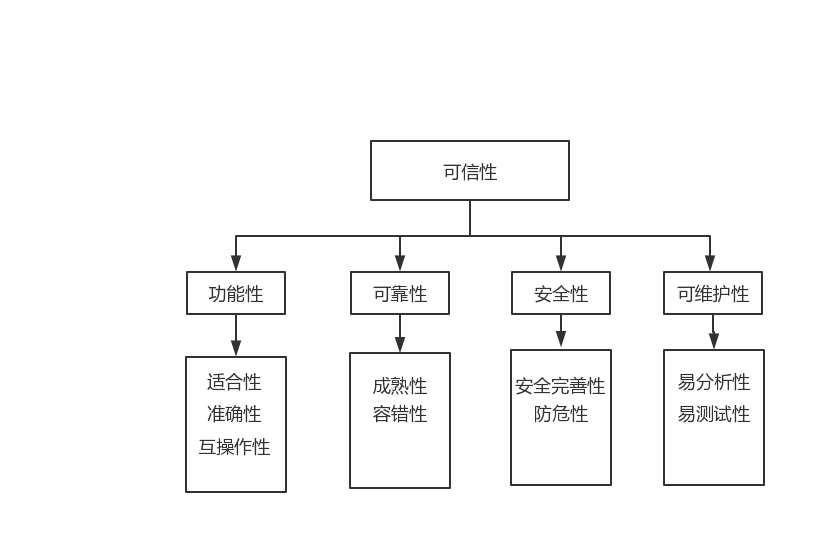
\includegraphics[width=13cm]{fig/2_01.png}\\
	\caption{轨道交通联锁软件可信属性分层模型}
	\label{fig:2_01}
\end{figure}

子属性向下进一步分解为更低层次的度量元,用来计算度量元可信值的数据称为可信证据。这些证据可以从软件源码,项目文档如需求说明书、设计文档和测试文档等,还有一些其他记录软件开发过程的文件中获取\cite{王德鑫2018支持软件过程可信评估的可信证据}。

\subsection{软件可信度量模型与分级方法}
文献\cite{王婧2015航天嵌入式软件可信性度量方法及应用研究}提出了航天型号软件可信性度量与评估体系,将度量元分为两种,将子属性的可信度划分为四个等级,从A到D依次递减。子属性的可信级别由专家给出,属性的可信度由下列公式计算得出:
\begin{equation}
y_i=Z_{i1}^{\beta_{i1}}\cdot Z_i2^{\beta_{i2}}\cdots Z_{i{w_i}}^{\beta_{i{w_i}}}
\end{equation}
其中,$y_i$为第i个属性的可信度值,$Z_{ij}$表示第i个属性的第j个子属性可信度值,$\beta_{ij}$为第i个属性中第j个子属性所占权重。
可信性度量计算模型为:
\begin{align}
\left\{
\begin{array}{lr}
\alpha_1+\alpha_2+\cdots +\alpha_n = \sum_{i=1}^n \alpha_i = 1 ~& 0 \leq \alpha_i \leq 1\\
T=y_1^{\alpha_1}y_2^{\alpha_2}\cdots y_n^{\alpha_n}=\prod_{i=1}^n y_i^{\alpha_i} ~& 0\leq y_i \leq 1
\end{array}
\right.
\end{align}
其中,T为软件可信度,$y_i$为第i个属性的可信度,$\alpha_i$为第i个属性的权重值。该模型满足“木桶原理”,必须保证每个属性的可信度值满足一定的条件,总体可信度才能达到要求。
这就类似于物理学科中的串联电路,属性可看作电路中的单一的元器件,任意一个单元都能决定该电路是否能连通。
% 可以将模型中各属性形象地理解为电路设计中构成串联关系的元器件。

本文的软件可信度量模型与分级方法在\cite{王婧2015航天嵌入式软件可信性度量方法及应用研究,伍志强2019基于可信证据的软件可信性计算模型设计与工具实现}的基础上,从四个阶段自下而上地计算度量元、子属性、属性、阶段到软件产品的可信值,进行可信等级划分。
第i个度量元可信值$x_i$的取值范围为[0,10],分两种类型的度量元,定性的度量元可信值根据打分得来,定量度量元可信值计算如下:
\begin{equation}
    x_i=(1-\frac{n}{m})*10
\end{equation}
其中,m为相关文档中规定该项度量元需完成的全部的任务数量,n为实际未完成的任务数量。
\begin{equation}
    y_i=\sum_{j=1}^n x_{ij}*{\alpha_{ij}} \label{formula:zishuxingkexinzhi}
\end{equation}

$x_{ij}$为第i个子属性中第j个度量元,$\alpha_{ij}$为第i个子属性中第j个度量元所占权重,$y_i$为第i个子属性的可信值。

\begin{equation}
    z_i=\prod_{j=1}^n y_{ij}^{\beta_{ij}} \label{formula:shuxingkexinzhi}
\end{equation}

$y_{ij}$为第i个属性中第j子属性,$\beta_{ij}$为第i个属性中第j个子属性所占权重,$z_i$为第i个属性的可信值。

\begin{equation}
    p_i=\prod_{j=1}^n z_{ij}^{\gamma_{ij}} \label{formula:jieduankexinzhi}
\end{equation}

$z_{ij}$为第i阶段中第j个属性,$\gamma_{ij}$为第i阶段中第j个属性所占权重,$p_i$为第i阶段的可信值。共有四个阶段。

\begin{equation}
    T=\prod_{i=1}^4 p_{i}^{w_{i}} \label{formula:ruanjiankexinzhi}
\end{equation}

软件的可信值为T,$w_i$为第i阶段所占的权重。

本文对\cite{伍志强2019基于可信证据的软件可信性计算模型设计与工具实现}进行修改,制定了适用于联锁软件的可信量化分级模型表,如\ref{tab-2-1}:
\begin{table}[!ht]
	\centering
	\renewcommand\arraystretch{1.3}
	\caption{可信量化分级模型表}
	\begin{tabular}{|c|c|c|c|}
		\hline
		\diagbox[width=8em,trim=l]{可信等级}{约束目标} & \textbf{\tabincell{c}{软件最低\\可信值}} & \textbf{\tabincell{c}{阶段可信值要求}} & \textbf{\tabincell{c}{属性可信值要求}}\\
		\hline
		  \textbf{\uppercase\expandafter{\romannumeral5}} & 9.5 & \tabincell{c}{最低8.5 且可信值低于\\9.5的阶段不超过1个}  & \tabincell{c}{最低8.5 且可信值低于\\9.5的属性不超过1个}  \\
		  \hline
		  \textbf{\uppercase\expandafter{\romannumeral4}} & 8.5 & \tabincell{c}{最低7.0 且可信值低于\\8.5的阶段不超过1个}  & \tabincell{c}{最低7.0 且可信值低于\\8.5的属性不超过1个}   \\
		  \hline
		  \textbf{\uppercase\expandafter{\romannumeral3}} & 7.0 & \tabincell{c}{最低4.5 且可信值低于\\7.0的阶段不超过1个}  & \tabincell{c}{最低4.5 且可信值低于\\7.0的属性不超过1个}   \\
		  \hline
		  \textbf{\uppercase\expandafter{\romannumeral2}} & 4.5 & \tabincell{c}{可信值低于4.5的\\阶段不超过1个} & \tabincell{c}{可信值低于4.5的\\属性不超过1个} \\
		  \hline
		  \textbf{\uppercase\expandafter{\romannumeral1}} & 1 & 无要求 & 无要求 \\ 
		\hline
	
	\end{tabular}
	\label{tab-2-1}
\end{table}


\section{结构方程模型的原理}
\subsection{结构方程模型的概念}
结构方程模型(SEM)又称为潜在变量模型(LVM),它是一种验证性的分析方法,
能够同时处理测量与分析的问题并非常重视多统计指标的运用,可以分析多个变量之间的影响关系以及变量和观测指标的一致性程度\cite{2004结构方程模型及其应用}。
软件可信性评估包括功能性、可靠性、安全性和可维护性,四个可信属性之间是有内在联系的,所以运用结构方程模型是比较合理的选择,并且该方法允许测量误差的存在\cite{王玖河2017顾客参与价值共创机理研究——基于结构方程模型的量化分析}。
该模型可以解决可信属性作为抽象的概念,无法直接观测或测量,也无法以数据量化来呈现的问题,在实际软件可信性评估中,是非常可取的。

结构方程模型由结构模型和测量模型两部分构成,前者是描述潜变量间的因果关系,后者是反映潜变量和观测变量之间的关系。
潜变量是构念因素,不可直接测量或无法直接观察得到,像学习动机、智力、学业成就等\cite{周涛2006结构方程模型及其在实证分析中的应用}。潜变量分为外因潜变量和内因潜变量,外因潜变量指模型中未受任何其他变量的影响,
而它却直接影响别的变量的变量,受到任一变量影响的变量称为内因潜变量。
观测变量又称显性变量、指标变量,可直接观察或测量获得,获得数据可被量化,比如语文、数学、外语三科成绩可作为学业成绩(潜变量)的测量变量\cite{周涛2006结构方程模型及其在实证分析中的应用}。

通常用LISREL和AMOS分析SEM,本文选择使用AMOS,原因如下:AMOS隶属SPSS系列,数据可以互用;AMOS界面简单,用户容易上手;AMOS得到的报表对用户来说相对容易解读\cite{吴明隆2010结构方程模型}。

\subsection{结构方程模型的结构}
(1)测量模型

% 下面方程用来描述潜变量与观测指标之间的关系\cite{程开明2006结构方程模型的特点及应用}:
如下方程表示潜变量与观测指标之间的关系\cite{周涛2006结构方程模型及其在实证分析中的应用}:

\begin{equation}
    x=\Lambda_x\xi+\delta \label{formula:x}
\end{equation}

\begin{equation}
    y=\Lambda_y\eta+\varepsilon \label{formula:y}
\end{equation}

x和y表示指标变量组成向量;$\Lambda_x$和$\Lambda_y$分别表示潜变量与指标变量之间的关系,称为指标变量在潜变量上的因子负荷矩阵;$\xi$和$\eta$分别为外因潜变量和内因潜变量;$\delta$和$\varepsilon$为指标变量的测量误差\cite{吴明隆2010结构方程模型}。

(2)结构模型

潜变量之间的关系用如下方程刻画\cite{程开明2006结构方程模型的特点及应用}:
\begin{equation}
    \eta=B\eta+\Gamma\xi+\zeta
\end{equation}

其中,B为内因潜变量之间的关系;$\Gamma$为外因潜变量对内因潜变量的影响;$\zeta$为结构方程的残差项,反映了$\eta$在方程中未能被解释的部分\cite{邹德玲2016网络嵌入视角下KIBS企业服务创新绩效影响机制研究}。

\section{系统开发框架与技术}
本文开发的轨道交通联锁软件可信测评系统基于web端,使用后台开发语言为Java,框架是Springboot,它可以帮助开发者快速搭建Spring框架,
简化配置文件的操作,开发人员主要将精力集中在业务逻辑实现上即可\cite{Gutierrez2017Spring},
%使编码、配置、部署和监控变得简单,极大地提高了开发和部署的效率\cite{Gutierrez2017Spring}。
视图层使用Spring推荐的Thymeleaf取代JSP作为模板渲染引擎。
其模板的HTML文件实现了前后端分离,在和后端无连接的情况下也可直接在浏览器中打开,显示文本内容,成功获取后端数据会取代默认文本渲染在页面上\cite{2012Spring}。
数据库使用了Mybatis框架,配置文件写好之后不需要在java代码中写SQL查询语句,简单易学,
因为不会对应用程序或者现有的数据库设计产生任何影响,可以降低代码和持久层的耦合。
实现相关图表展示功能时用到了第三方插件Echarts库,其中包含丰富的图表类型可供选择,用户还可以根据自己的业务需求,自定义图表显示内容。



\section{本章小结}
本章内容涉及三个方面。第一方面是软件可信性的相关概念,如软件可信性定义,软件可信属性、子属性、度量元,可信度量模型。第二方面介绍了结构方程模型的原理。最后一方面阐释了相关技术点在工具开发中的应用。

\label{ch2}



